% MultiSpec-GeoDiff Demo Report — Polished LaTeX
% Compile: latexmk -xelatex demo_report.tex
\documentclass[11pt,a4paper]{ctexart}

% ── Packages ──
\usepackage[margin=0.85in]{geometry}
\usepackage{graphicx}
\usepackage{booktabs}
\usepackage[table]{xcolor}
\usepackage{tcolorbox}
\usepackage{hyperref}
\usepackage{amsmath}
\usepackage{caption}
\usepackage{subcaption}
\usepackage{fancyhdr}
\usepackage{enumitem}
\usepackage{fontspec}

% ── CJK font fallback ──
\setCJKmainfont{SimSun}[AutoFakeBold=2.5]
\setCJKsansfont{SimSun}[AutoFakeBold=2.5]
\setCJKmonofont{SimSun}

% ── Colors ──
\definecolor{darkblue}{HTML}{1a1a2e}
\definecolor{midblue}{HTML}{2c5f8a}
\definecolor{lightblue}{HTML}{4a90c4}
\definecolor{bgblue}{HTML}{e8f0f8}
\definecolor{greytext}{HTML}{555555}
\definecolor{lightgrey}{HTML}{aaaaaa}
\definecolor{greenok}{HTML}{2d7a4f}

% ── tcolorbox styles ──
\newtcolorbox{infobox}{
  colback=bgblue, colframe=midblue, arc=3mm, boxrule=0.6pt,
  left=8pt, right=8pt, top=6pt, bottom=6pt,
  before skip=4pt, after skip=10pt
}
\newtcolorbox{scopebox}{
  colback=blue!4!white, colframe=midblue, arc=3mm, boxrule=0.8pt,
  left=10pt, right=10pt, top=8pt, bottom=8pt,
  before skip=4pt, after skip=10pt
}

% ── Header / footer ──
\pagestyle{fancy}
\fancyhf{}
\fancyfoot[C]{\small\color{greytext} MultiSpec-GeoDiff Demo \textbar\ DP Technology Internship \textbar\ \thepage}
\renewcommand{\headrulewidth}{0pt}
\renewcommand{\footrulewidth}{0.3pt}

% ── Compact lists ──
\setlist{nosep,leftmargin=*,itemsep=0pt,topsep=2pt,partopsep=0pt}

% ── Hyperref setup ──
\hypersetup{
  colorlinks=true,
  linkcolor=midblue,
  urlcolor=midblue,
  citecolor=midblue,
  pdfauthor={MultiSpec-GeoDiff},
  pdftitle={MultiSpec-GeoDiff — Demo Description}
}

% ── Title formatting ──
\newcommand{\demotitle}{
  \begin{center}
    {\LARGE\bfseries\color{darkblue} MultiSpec-GeoDiff}\\[4pt]
    {\large\bfseries\color{midblue} Stage-I Feasibility Loop}\\[2pt]
    {\normalsize\color{greytext} 多模态谱图驱动的几何分子结构反演 \textbar\ Demo 说明}\\[6pt]
    \rule{0.6\textwidth}{0.4pt}\\[6pt]
  \end{center}
}

\begin{document}

% ======================================================================
% TITLE
% ======================================================================
\demotitle

% ======================================================================
% INFO CARD (first thing on page 1)
% ======================================================================
\begin{infobox}
\small
\begin{tabular}{@{}p{0.22\textwidth} p{0.75\textwidth}@{}}
  \textbf{项目名称} &
    MultiSpec-GeoDiff: Multimodal Spectra-Driven Geometric Molecular Structure Inversion \\[3pt]
  \textbf{提交类型} &
    DP Technology 实习项目 Demo \\[3pt]
  \textbf{当前阶段} &
    Stage-I 可行性闭环 \\[3pt]
  \textbf{实验数据} &
    200 条 NIST 实验 IR 光谱 \\[3pt]
  \textbf{仓库地址} &
    \url{https://github.com/techandscixie2005/MultiSpec-GeoDiff-Demo} \\[3pt]
  \textbf{一键运行} &
    \texttt{python 03\_code/run\_demo.py --query\_id 0 --data 04\_data/IR\_nist\_200.jsonl --top\_k 5} \\[3pt]
  \textbf{测试命令} &
    \texttt{PYTHONPATH=03\_code/src pytest 03\_code/tests -q} \\[3pt]
  \textbf{验证状态} &
    22 个测试通过 \textbar\ GitHub Actions CI 通过
\end{tabular}
\end{infobox}

% ======================================================================
% SECTION 1: TASK GOAL
% ======================================================================
\section{任务目标、定位与价值}

分子光谱到结构的反演是 AI for Science 领域典型的逆问题。实验红外光谱存在噪声、稀疏性和一谱多解的内在歧义，直接生成 SMILES 字符串忽视了分子的图拓扑与三维几何结构。本项目提议将反演形式化为多阶段条件生成问题；本 Demo 聚焦于 \textbf{Stage-I 最小可行性闭环}。

核心管线为：
\begin{center}
\begin{tcolorbox}[colback=bgblue, colframe=midblue, arc=2mm, boxrule=0.4pt,
  width=0.92\textwidth, halign=center]
\small
\textbf{实验 IR 光谱}
$\;\rightarrow\;$ 坐标感知谱图编码
$\;\rightarrow\;$ 候选检索
$\;\rightarrow\;$ 前向谱图重排
$\;\rightarrow\;$ \textbf{Top-K 候选分子}
\end{tcolorbox}
\end{center}

\textbf{定位说明：} 本 Demo 不是训练完备的生成模型，也不是生产级未知物鉴定系统。它展示的是一个可追溯的 AI-for-Science 工作流——在真实实验数据上验证``候选提出 + 前向一致性校验''的闭环思想，符合实习项目对可行性、逻辑推理与创新性展示的要求。

% ======================================================================
% SECTION 2: CORE CAPABILITIES
% ======================================================================
\section{已完成核心能力}

\begin{table}[ht]
\small
\begin{tabular}{@{}p{0.28\textwidth} p{0.38\textwidth} p{0.30\textwidth}@{}}
\toprule
\bfseries 能力模块 & \bfseries 当前 Demo 状态 & \bfseries 仓库证明材料 \\
\midrule
NIST IR 数据加载 & 已实现 & \texttt{04\_data/IR\_nist\_200.jsonl} \\
谱图插值与归一化 & 已实现 & \texttt{spectra\_preprocess.py} \\
坐标感知谱图编码 & 已实现 & \texttt{spectra\_encoder.py} \\
谱图距离偏置注意力 & 已实现 & \texttt{spectral\_attention.py}, 热图 \\
候选分子检索 & 已实现 & \texttt{candidate\_generator.py} \\
前向谱图重排 & 已实现 & \texttt{reranker.py} \\
Top-K 输出与可视化 & 已实现 & CSV, PNG 输出文件 \\
可追溯 Demo 日志 & 已实现 & \texttt{trace\_log.json} \\
本地测试与 CI & 已实现 & 22 测试, GitHub Actions \\
\rowcolor{blue!3!white}
Pairwise 距离预测头 & 接口原型 & \texttt{distance\_head.py} \\
\rowcolor{blue!3!white}
TFN/SE(3) 等变模块 & 接口原型 & \texttt{tfn\_transformer\_stub.py} \\
\bottomrule
\end{tabular}
\end{table}

\vspace{-4pt}
{\small\color{greytext} 200 条 NIST 实验 IR 光谱用于 Demo 级可行性验证，未用于训练完整生成模型。}

% ======================================================================
% SECTION 3: WORKFLOW & OUTPUTS
% ======================================================================
\section{Demo 工作流与输出示例}

\begin{figure}[ht]
\centering
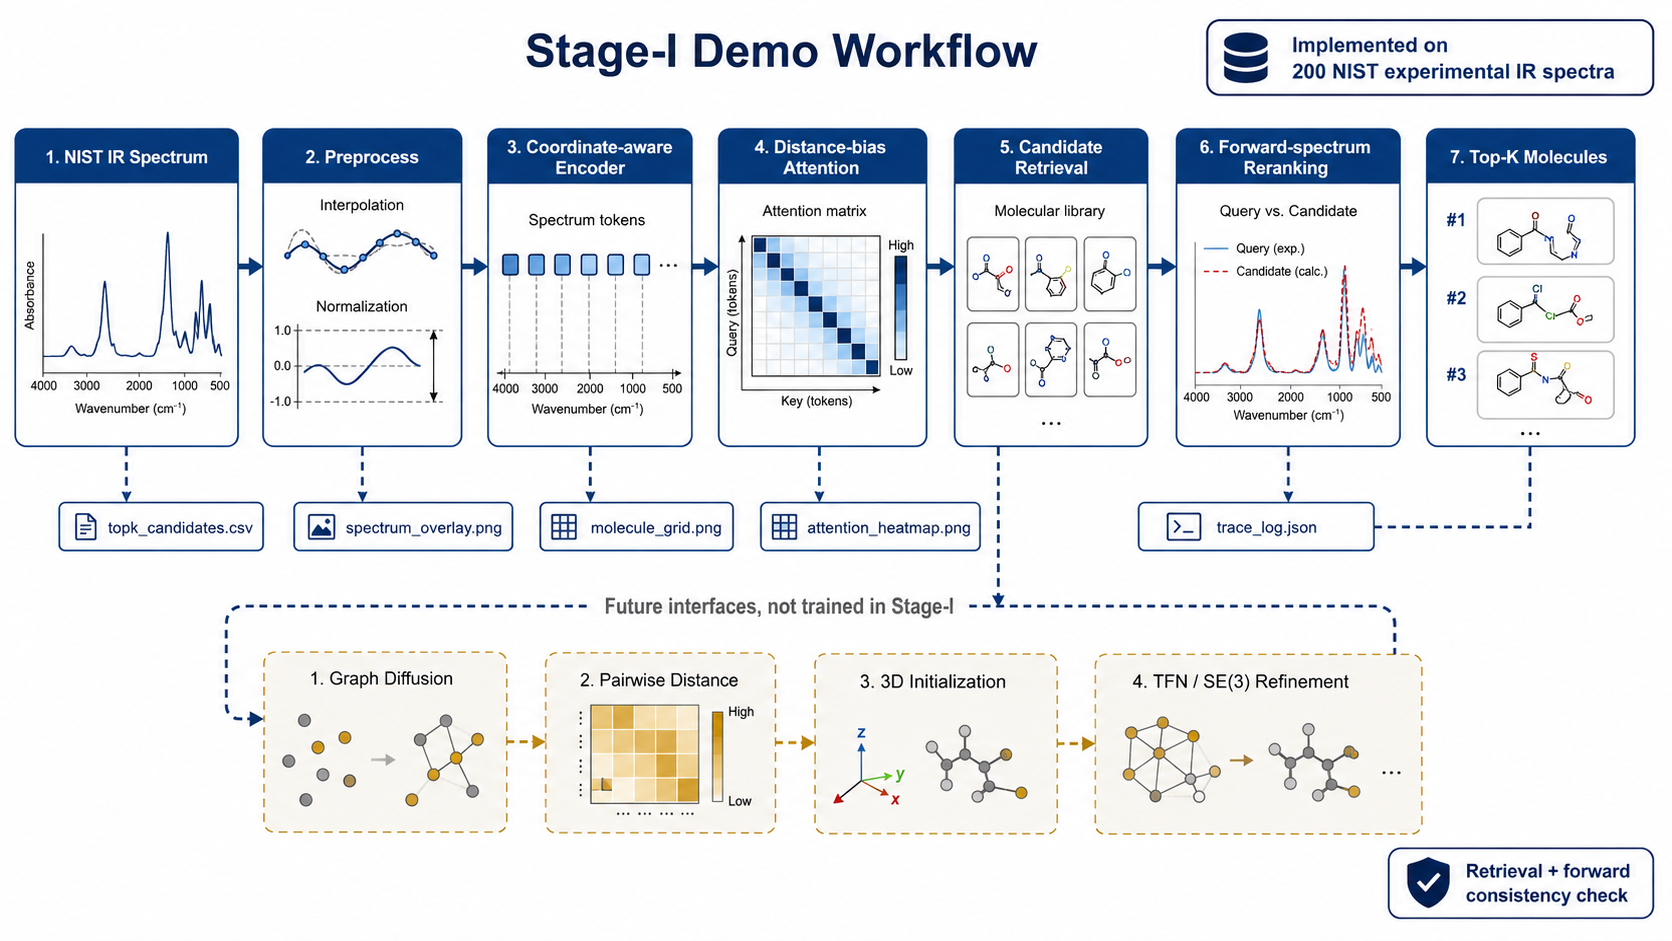
\includegraphics[width=0.98\linewidth]{figures/stage1_workflow.png}
\caption{Stage-I Demo 工作流。实心蓝色模块为已实现的 Stage-I 检索/重排闭环（200 条 NIST 实验 IR 光谱）；虚线模块为图扩散、pairwise 距离预测及 TFN/SE(3) 等变细化的未来接口，非本 Demo 已完成功能。}
\label{fig:workflow}
\end{figure}

\subsection{输入与输出}

\begin{table}[ht]
\small
\begin{tabular}{@{}p{0.10\textwidth} p{0.42\textwidth} p{0.44\textwidth}@{}}
\toprule
& \bfseries 输入 & \bfseries 输出 \\
\midrule
\textbf{数据} &
  \texttt{04\_data/IR\_nist\_200.jsonl}\newline
  每条含 SMILES / 波数 / 强度 &
  \texttt{05\_outputs/topk\_candidates.csv}\newline
  \texttt{05\_outputs/spectrum\_overlay.png}\newline
  \texttt{05\_outputs/molecule\_grid.png}\newline
  \texttt{05\_outputs/attention\_heatmap.png}\newline
  \texttt{05\_outputs/ablation\_results.csv}\newline
  \texttt{05\_outputs/trace\_log.json} \\
\textbf{参数} &
  \texttt{query\_id = 0}\newline
  \texttt{top\_k = 5} & \\
\bottomrule
\end{tabular}
\end{table}

\subsection{输出示例}

\begin{figure}[ht]
\centering
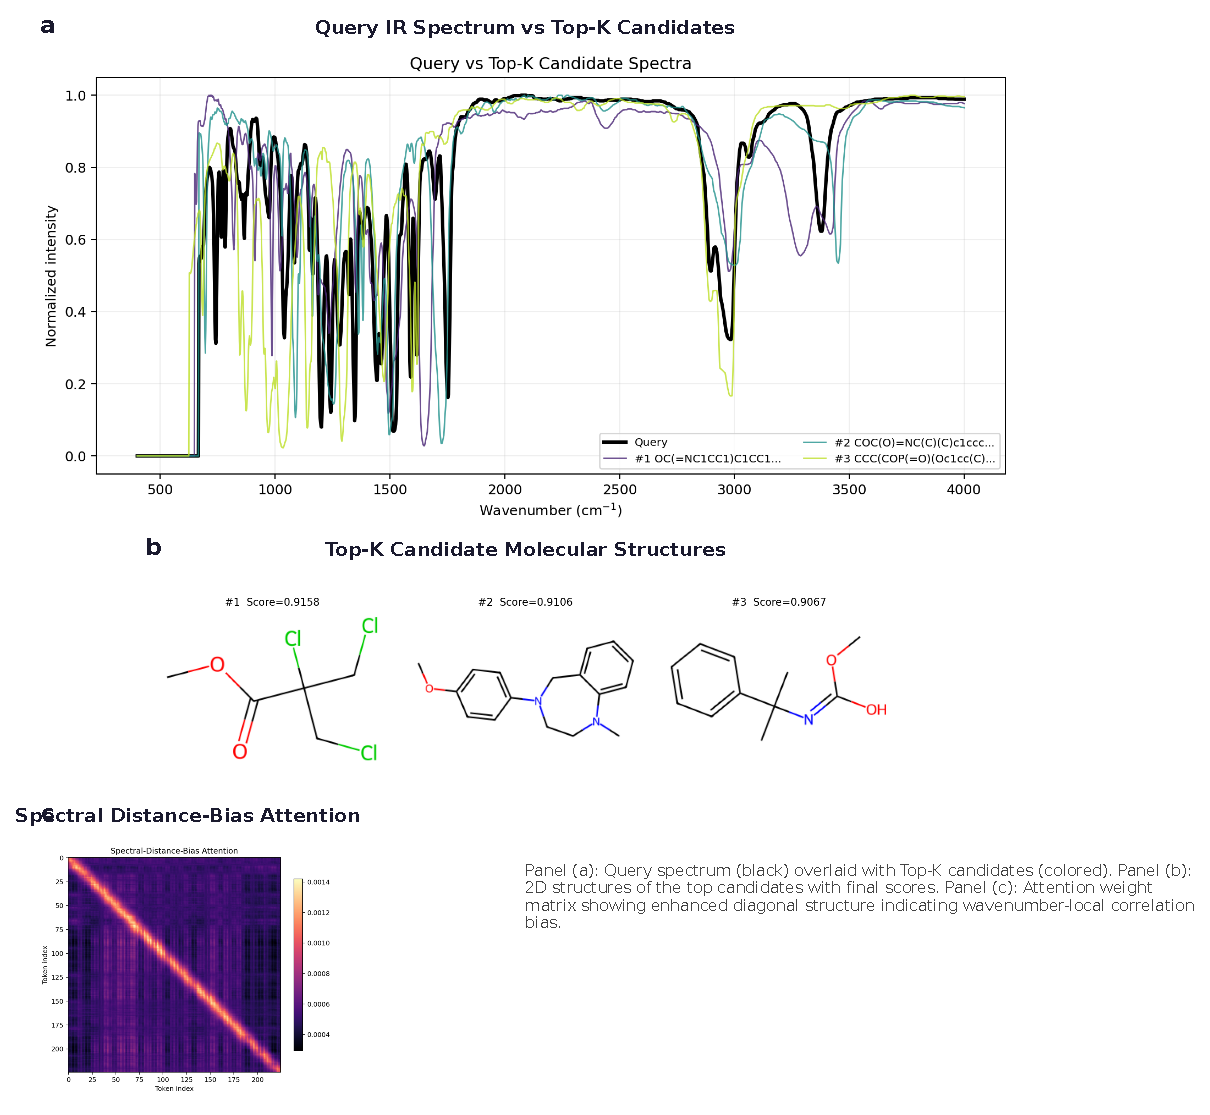
\includegraphics[width=\textwidth]{figures/fig2_outputs.pdf}
\caption{Demo 输出示例。\textbf{(a)} 查询光谱（黑色）与 Top-K 候选（彩色）叠加对比。\textbf{(b)} Top-K 候选分子二维结构及得分。\textbf{(c)} 谱图距离偏置注意力热图，对角线增强表明波数邻近区域具有更强局部相关性。}
\label{fig:outputs}
\end{figure}

% ======================================================================
% SECTION 4: CORE PRINCIPLE
% ======================================================================
\section{核心原理}

\subsection{坐标感知谱图编码}

\begin{equation}\label{eq:embed}
h_i = W_I \cdot I_i + p(\nu_i)
\end{equation}

IR 光谱的每个数据点不是无结构的序列 token——它同时携带强度信息 $I_i$ 与波数物理坐标 $\nu_i$。嵌入层将强度投影与傅里叶波数位置编码相加，使模型天然地感知每个点位于光谱的哪个位置。这是本 Demo 区别于普通 Transformer 序列编码的核心设计。

{\small\color{midblue}\textbf{核心思路：} IR 波数轴被视作物理坐标，而非无结构序列索引。}

\subsection{谱图距离偏置注意力}

\begin{equation}\label{eq:attn}
A_{ij} = \operatorname{softmax}_j\left(\frac{Q_i K_j^T}{\sqrt{d}} + b(|\nu_i - \nu_j|)\right)
\end{equation}

在 IR 光谱中，物理上邻近的波数区域具有更强的本征相关性——这一先验不应由模型从有限数据中从头学习。本设计在注意力中注入波数间距依赖的 RBF 偏置 $b(\Delta\nu) = \exp(-(\Delta\nu/\sigma)^2)$，使远离谱区之间的注意力权重被物理先验抑制。这与 Graph Transformer 中注入拓扑距离偏置的思路一致，但应用对象是\textbf{光谱物理坐标}。

{\small\color{midblue}\textbf{核心思路：} 注意力被物理谱距偏置，而非仅依赖 token 相似度。}

\subsection{候选检索与前向谱图重排}

\begin{equation}\label{eq:score}
\operatorname{Score}(G_k) = \lambda_1 \operatorname{CosSim}(S_q, S_k) + \lambda_2 \operatorname{PeakMatch}(S_q, S_k)
\end{equation}

当前 Demo 使用检索而非训练完成的图扩散模型来产生候选——这是 Stage-I 的刻意简化。检索后，候选分子经前向谱图对比进行三指标重排（余弦相似度 + L1 距离 + 峰匹配），验证``候选提出 + 前向一致性校验''的闭环在真实实验数据上的可行性。在后续阶段，检索模块可替换为谱图条件图扩散生成。

{\small\color{midblue}\textbf{核心思路：} 候选分子通过前向谱图一致性进行重排，而非仅依赖嵌入相似度。}

% ======================================================================
% SECTION 5: SCOPE BOUNDARY
% ======================================================================
\section{能力边界}

\begin{scopebox}
\small
\textbf{当前 Demo 已实现：}
\begin{itemize}
  \item Stage-I IR 检索与重排可行性闭环（200 条 NIST 实验 IR 光谱）
  \item 坐标感知谱图编码（将波数轴视为物理坐标）
  \item 谱图距离偏置注意力（基于物理谱距而非 token 相似度）
  \item 候选分子检索与前向谱图重排
  \item 可视化输出（谱图叠加、分子网格、注意力热图）
  \item 可追溯执行日志（\texttt{trace\_log.json}）
  \item 本地测试与 GitHub Actions CI（22 个测试全部通过）
\end{itemize}

\vspace{4pt}
\textbf{当前 Demo 未包含：}
\begin{itemize}
  \item 未训练完整的图扩散生成模型
  \item 未训练完整的 pairwise 距离预测器
  \item 未训练完整的宇称分辨 TFN/SE(3)-Transformer
  \item 未接入 IR/Raman/NMR/MS/UV 等多模态谱图系统
  \item 未建立生产级未知物鉴定系统
\end{itemize}
\end{scopebox}

{\small\color{greytext} 这一边界是刻意的。Demo 的目标是展示核心思路与可行性闭环，而非交付完整的生产系统。Stage-II 和 Stage-III 的关键模块已作为可导入接口桩存在于代码库中，定义了清晰的接口签名与数据结构。}

% ======================================================================
% SECTION 6: VALIDATION
% ======================================================================
\section{验证结果与价值}

\begin{table}[ht]
\small
\begin{tabular}{@{}p{0.22\textwidth} p{0.74\textwidth}@{}}
\toprule
\bfseries 项目 & \bfseries 状态 \\
\midrule
实验数据 &
  200 条 NIST 实验 IR 光谱（\texttt{04\_data/IR\_nist\_200.jsonl}）\\
Demo 命令 &
  \texttt{python 03\_code/run\_demo.py --query\_id 0 \dots\ --top\_k 5} \\
本地测试 &
  22 个测试全部通过（pytest）\\
CI &
  GitHub Actions Tests 通过 \\
关键输出 &
  Top-K CSV、谱图叠加、分子网格、注意力热图、trace log \\
消融验证 &
  流程各模块可独立开关和记录；Full pipeline 在余弦相似度之外引入 L1 与峰匹配信号 \\
\bottomrule
\end{tabular}
\end{table}

\vspace{-4pt}
\textbf{Demo 的核心价值可概括为三点：}
\begin{enumerate}[nosep]
  \item 证明了真实实验 IR 光谱可以进入可复现的检索/重排闭环。
  \item 证明了坐标感知谱图注意力是可实现的，并可作为后续阶段的编码器基础。
  \item 为检索$\rightarrow$图扩散$\rightarrow$几何细化的逐步替换提供了清晰的代码接口。
\end{enumerate}

{\small\color{greytext}\textbf{消融说明：} 当前消融主要用于验证流程各模块可被独立开关和记录，非统计显著性能声明。由于样本规模仅 200，结果应理解为 Demo 级可行性检验。Full pipeline 在纯余弦相似度之外引入 L1 与峰匹配信号，使候选排序更接近谱图物理一致性。}

% ======================================================================
% SECTION 7: ROADMAP
% ======================================================================
\section{后续演进路线}

本 Demo 聚焦于 Stage-I 可行性验证；Stage-II 与 Stage-III 为计划中的未来扩展方向，当前代码库中保留接口定义但未包含完整训练的生成模型。

\begin{figure}[ht]
\centering
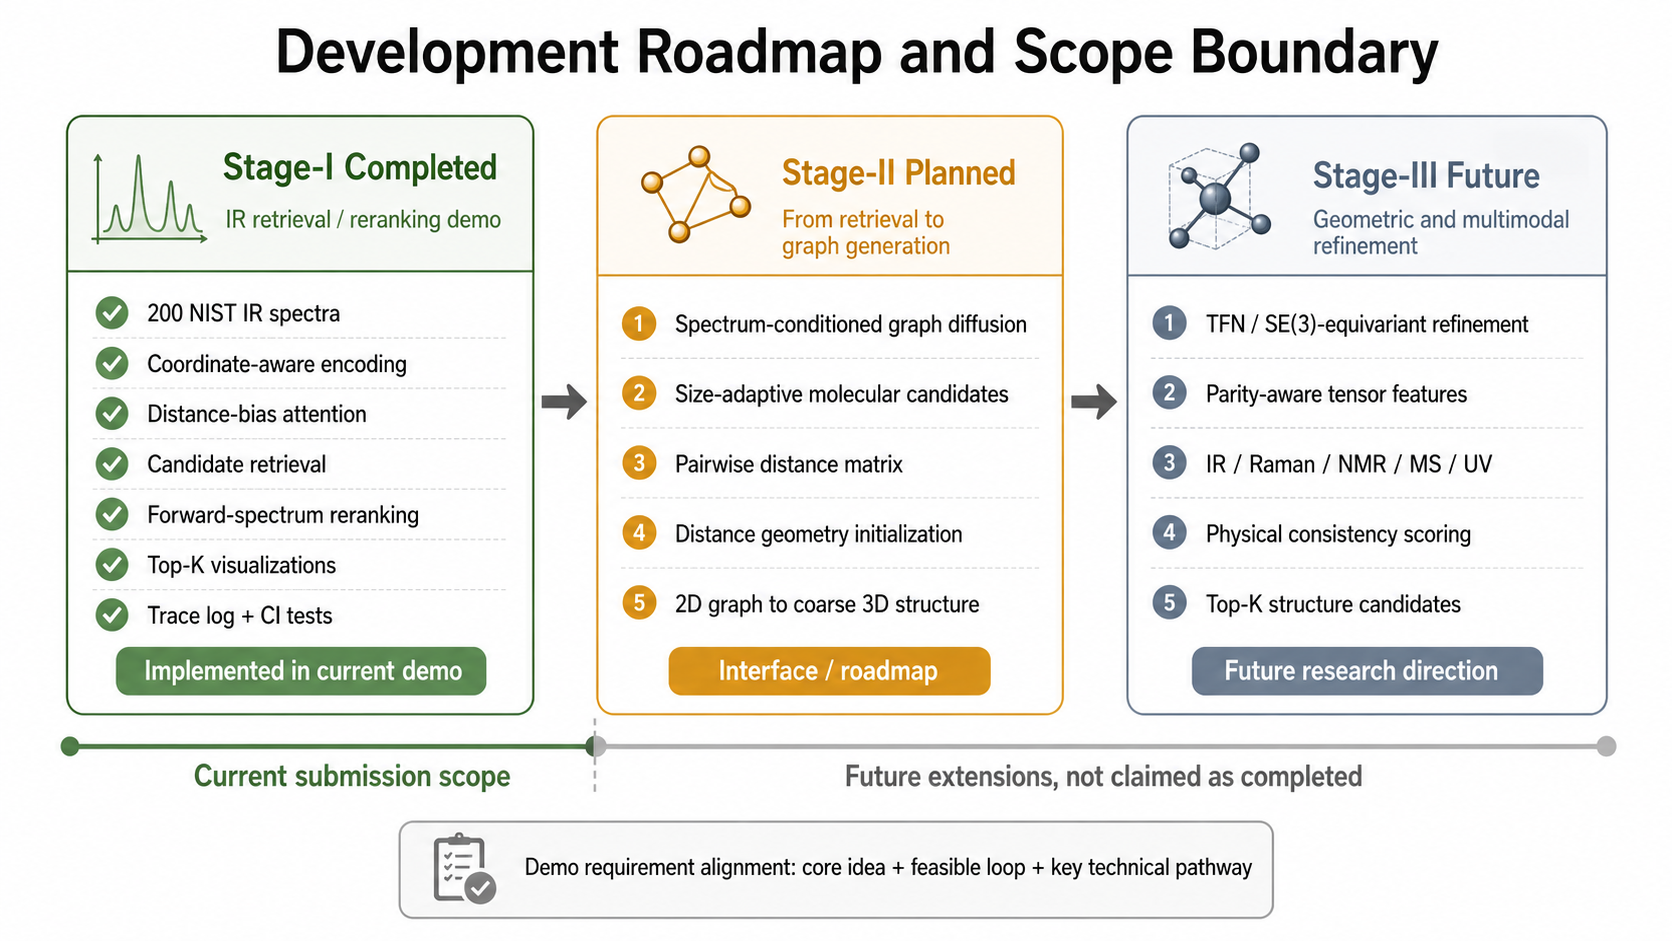
\includegraphics[width=0.98\linewidth]{figures/roadmap.png}
\caption{开发路线图与能力边界。Stage-I 为本提交已完成内容；Stage-II 与 Stage-III 为计划中的未来扩展。当前 Demo 验证的是可行性闭环思想，而非完整训练的分子生成模型。}
\label{fig:roadmap}
\end{figure}

% ======================================================================
% SECTION 8: SUBMISSION CHECKLIST
% ======================================================================
\section{提交材料清单}

\begin{table}[ht]
\small
\begin{tabular}{@{}p{0.24\textwidth} p{0.72\textwidth}@{}}
\toprule
\bfseries 材料 & \bfseries 路径 \\
\midrule
GitHub 仓库 &
  \url{https://github.com/techandscixie2005/MultiSpec-GeoDiff-Demo} \\
项目提议 &
  \texttt{01\_project\_proposal/proposal.md} \\
Demo 说明 PDF &
  \texttt{02\_demo\_document/demo\_report.pdf}（本文档）\\
LaTeX 源码 &
  \texttt{02\_demo\_document/latex/demo\_report.tex} \\
代码 &
  \texttt{03\_code/}（核心模块 + 测试 + CLI 入口）\\
数据 &
  \texttt{04\_data/IR\_nist\_200.jsonl}（200 条 NIST IR 光谱）\\
输出 &
  \texttt{05\_outputs/}（CSV, PNG, JSON）\\
Notebook &
  \texttt{06\_notebook/demo\_pipeline.ipynb} \\
CI &
  \texttt{.github/workflows/tests.yml} \\
\bottomrule
\end{tabular}
\end{table}

\vspace{6pt}
\begin{center}
{\small\color{greytext}
\textbf{主命令：} \texttt{python 03\_code/run\_demo.py --query\_id 0 --data 04\_data/IR\_nist\_200.jsonl --top\_k 5} \\
\textbf{测试命令：} \texttt{PYTHONPATH=03\_code/src pytest 03\_code/tests -q} \\
仓库地址：\url{https://github.com/techandscixie2005/MultiSpec-GeoDiff-Demo}
}
\end{center}

\end{document}
